% !TEX root = main.tex

\documentclass[aspectratio=169,11pt,xcolor={dvipsnames},hyperref={pdftex,pdfpagemode=UseNone,hidelinks,pdfdisplaydoctitle=true},usepdftitle=false]{beamer}
\usepackage{../include/slide}
\usepackage{tikz}


\title{Lean Applications in the Department of Defense}
\author{Juan Carlos Cruz - ira406}
\date{ME 5703 Lean Product Development and Service Systems}

\begin{document}
    
    \begin{frame}
      \titlepage
      May 2025
    \end{frame}
    
    \begin{frame}{Introduction}
      \begin{itemize}
        \item DoD traditionally viewed as bureaucratic and slow-moving
        \item Study investigates lean/six-sigma implementation within DoD
        \item Scientometric review of 465 documents (1992-2025)
        \item Case study examination of notable works from the dataset and out of dataset example
      \end{itemize}
    \end{frame}

    \begin{frame}{Literature Search}
      \begin{itemize}
        \item In ProQuest create a search as:\\
          \begin{minipage}{\linewidth}
          \begin{spacing}{0.8}
          \noindent\texttt{AB("Department of Defense" OR "DoD" OR "DOD" OR "U.S. Army" OR} \\
          \texttt{"Department of the Army" OR "U.S. Navy" OR "Department of the Navy" OR} \\
          \texttt{"U.S. Air Force" OR "Department of the Air Force" OR "U.S. Marine Corps" OR} \\
          \texttt{"U.S. Space Force" OR "National Security Agency" OR "NSA" OR} \\
          \texttt{"Defense Intelligence Agency" OR "DIA" OR "National Geospatial-Intelligence} \\
          \texttt{Agency" OR "NGA" OR "National Reconnaissance Office" OR "NRO")} \\
          \texttt{AND FT("six sigma" OR "6$\sigma$" OR "lean six sigma" OR} \\
          \texttt{"continuous process improvement" OR "LSS") AND LA(EN)}
          \end{spacing}
          \end{minipage}
        \item 465 documents after cleaning are exported to a spreadsheet.
      \end{itemize}
    \end{frame}


    \begin{frame}{Scientometric Analysis}
      \begin{itemize}
        \item 2 step Python program to analyze publication trends and then classify themes
        \begin{enumerate}
          \item Analyze abstracts and publication data for trends then use Latent Dirichlet Analysis on abstract to extract themes
          \item When themes extracted create a list of lean keywords related to that theme (Ex. Process Improvement: process, improvement, quality...), and classify abstracts similarity to theme
        \end{enumerate}
        \item Publication trends: Increase from 1992-2017, decline after 2017
        \item Document types: Primarily Theses and Trade journals
        \item Three themes identified: Management (54\%), Process Improvement (36\%), Continuous Learning (9\%)
        \item From classified papers we now analyze some case studies
      \end{itemize}
    \end{frame}

    \begin{frame}{Scientometric Analysis - Graphs}

      \begin{columns}
        \begin{column}{0.48\textwidth}
          \begin{figure}
                \centering
                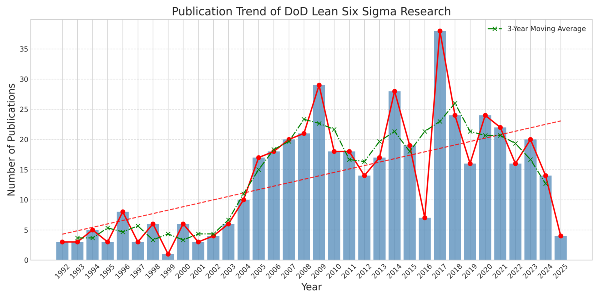
\includegraphics[width=\linewidth]{../figures/publication_trend.pdf}
              \end{figure}
          \end{column}
          
        \begin{column}{0.48\textwidth}
          \begin{figure}
                \centering
                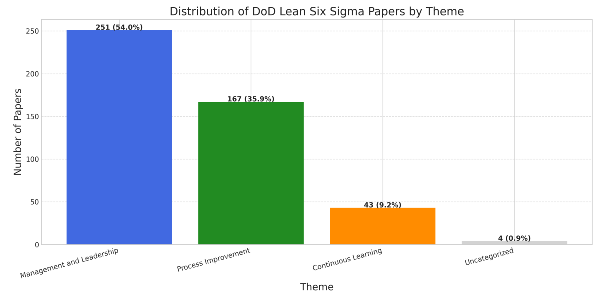
\includegraphics[width=\linewidth]{../figures/theme_distribution_bar.pdf}
              \end{figure}
          \end{column}
        \end{columns}

    \end{frame}

    \begin{frame}{Management and Leadership - Overview}
      \begin{itemize}
        \item Toyota's Hourensou vs. DoD's command-and-control
        \item Case studies show adaptation to DoD structures based on lean principles
        \item Case studies selected demonstrate lean for management of people and suppliers.
      \end{itemize}
    \end{frame}


    \begin{frame}{Management Case - Leadership Development \cite{McCants2024}}
      \begin{itemize}
        \item Study through interviews with senior leadership in Dept. of Army, Washington D.C. to reduce variability in leadership success for high turnover positions
        \item Five key themes identified for successful transitions:
          \begin{itemize}
            \item Knowledge of organization during change
            \item Effective communication skills
            \item Flexible and adaptive leadership
            \item Having performance measures
            \item Formal and informal leader development
          \end{itemize}
        \item Lean connection: \textit{genchi genbutsu} (go and see) and \textit{hourensou} communication
        \item Shows lean leadership applicable even in hierarchical military structures
      \end{itemize}
    \end{frame}

    \begin{frame}{Management Case - Project Engineer Stress \cite{Turner2024}}
      \begin{itemize}
        \item Study of work-related stressors and turnover among 69 DoD project engineers
        \item Through root cause analysis the author statistically correlated variables to turnover intention
        \item Key stress factors identified:
          \begin{itemize}
            \item Excessive workloads
            \item Tight deadlines
            \item Technical complexity
            \item Interpersonal conflict
            \item Insufficient resources
          \end{itemize}
        \item Lean connection: Addresses \textit{muri} (overburden) as key waste
        \item Demonstrates need for \textit{heijunka} (leveled workflow) in project management
      \end{itemize}
    \end{frame}

    \begin{frame}{Management Case - Contract Environment \cite{Carlstedt2020}}
      \begin{itemize}
        \item Analysis of Army supplier contract management process
        \item Structured approach using:
          \begin{itemize}
            \item Performance Work Statements (PWS)
            \item Contract Officer's Representatives (COR)
            \item Regular performance reviews (PMRs and CMRs)
          \end{itemize}
        \item Standardized documents and regular reviews create feedback loops for continuous improvement
        \item Balance between strict enforcement and contractor relationship
        \item Lean connection: Reflects Toyota's \textit{keiretsu} philosophy of building long-term supplier partnerships
      \end{itemize}
    \end{frame}


    \begin{frame}{Process Improvement - Overview}
      \begin{itemize}
        \item Process improvement fundamental to lean organizations
        \item Based on culture of \textit{kaisen} (continuous improvement)
        \item Focus on identifying and removing non-value adding steps (waste)
        \item Case studies demonstrate different approaches to process improvement in DoD
      \end{itemize}
    \end{frame}

    \begin{frame}{Process Improvement - Cost Analysis of Ceremonies \cite{Malin2020}}
      \begin{itemize}
        \item Study of Army's Change of Command (COC) ceremonies and associated costs
        \item Found Army lacks proper process to evaluate production loss costs:
          \begin{itemize}
            \item Company-sized unit: \$17,964 per hour
            \item Division-sized unit: \$404,200 per hour
          \end{itemize}
        \item Research led to development of cost tool to support decision-making
        \item Lean connection: Identifying hidden costs (muda) in traditional practices
      \end{itemize}
    \end{frame}

    \begin{frame}{Process Improvement - Depot Repair Lead Time \cite{Richmond2023}}
      \begin{itemize}
        \item Application of Lean Six Sigma to small government depot repair facility
        \item Analysis revealed 80\% of repair lead time attributed to non-value-added waiting
        \item Implementation included:
          \begin{itemize}
            \item Cross-training personnel
            \item Process swimlane improvements
            \item Standardized documentation
          \end{itemize}
        \item Results: 84\% decrease in lead times (114 days to 18 days)
        \item Lean connection: DMAIC methodology effectively applied to service operations
        \item Shows lean principles adaptable to maintenance service contexts
      \end{itemize}
    \end{frame}

    \begin{frame}{Process Improvement - DoD Contract Cost Overruns \cite{FunchesAllen2025}}
      \begin{itemize}
        \item Machine learning analysis of 524 DoD contracts to predict cost overruns
        \item Random forest model achieved 80\% accuracy in predictions
        \item Primary factors contributing to overruns:
          \begin{itemize}
            \item Inaccurate cost estimation (42\% of cases)
            \item Inadequate risk assessment (21.8\%)
            \item Scope modifications (11.8\%)
            \item Technical issues (6.1\%)
          \end{itemize}
        \item Lean connection: Cost overruns represent financial \textit{muda} (waste)
        \item Identification of key factors enables targeted \textit{kaizen} initiatives
      \end{itemize}
    \end{frame}


  \begin{frame}{Continuous Learning - Overview}
    \begin{itemize}
      \item Building culture of continuous learning (\textit{hansai} and \textit{kaisen}) is cornerstone of Toyota Way
      \item Digital age amplifies learning through data and knowledge management
      \item Poor information systems create waste if data not accessible at right time by right people
      \item Case studies show DoD efforts to improve knowledge management and data-driven learning
    \end{itemize}
  \end{frame}

  \begin{frame}{Continuous Learning - PTSD Diagnosis Tool \cite{Le2023}}
    \begin{itemize}
      \item Development of Classification Automation Tool (CAT) using machine learning for PTSD diagnosis
      \item Approaches diagnostic errors as form of waste in engineering terms
      \item Stacked ensemble machine learning achieved statistically significant reduction in misdiagnoses
      \item Identified ten key predictors connected with PTSD in veterans
      \item Lean connection: Reduces defects (misdiagnoses) in medical process
      \item Both false positives and false negatives represent different forms of \textit{muda} (waste)
    \end{itemize}
  \end{frame}

  \begin{frame}{Continuous Learning - Army Knowledge Management \cite{VanLaar2023}}
    \begin{itemize}
      \item Qualitative case study examining Army's knowledge management implementation
      \item Used two assessment tools: Knowledge Management Maturity Model (KM3) and Knowledge Management Assessment Tool (KMAT)
      \item Analysis revealed "people" component ranked lowest - tacit knowledge not properly shared
      \item Four knowledge transfer barriers identified:
        \begin{itemize}
          \item Content management issues
          \item Personnel turnover impacts
          \item Portal use and governance challenges
          \item Need for institutional governance
        \end{itemize}
    \end{itemize}
  \end{frame}

  \begin{frame}{Continuous Learning - Army Data Fabric \cite{Patel2021}}
    \begin{itemize}
      \item Implementation of data fabric technology to address data stovepipes and inefficient sharing
      \item Creates common layer for data discovery, synchronization and security across systems
      \item Critical challenges identified:
        \begin{itemize}
          \item Data isolation in warfighting functional systems
          \item Compression-induced information loss
          \item Unnecessarily restrictive classification
          \item AI capabilities unable to access needed data
        \end{itemize}
      \item Project Rainmaker developed as tactical data fabric solution
      \item Lean connection: Addresses digital \textit{muda} (waiting waste) with pull-based data system
    \end{itemize}
  \end{frame}



    \begin{frame}{Out of Sample Study - Defense Innovation Unit}
      \begin{columns}
        \begin{column}{0.48\textwidth}
          % Make itemize more compact
          \setlength{\itemsep}{0pt}
          \setlength{\parskip}{0pt}
          \begin{itemize}
            \item Established 2015 as DoD's gateway to tech companies
            \item Streamlined acquisition: 60-90 days vs. years
            \item Example: GigEagle
              % Make nested itemize more compact
              \setlength{\itemsep}{0pt}
              \setlength{\parskip}{0pt}
              \begin{itemize}
                \item Matches DoD with Reserve/Guard personnel for gigs
                \item Addresses waste: underutilized talent
                \item Lean approach to human capital management
              \end{itemize}
          \end{itemize}
        \end{column}
        
          
          \begin{column}{0.48\textwidth}
            \begin{figure}
                  \centering
                  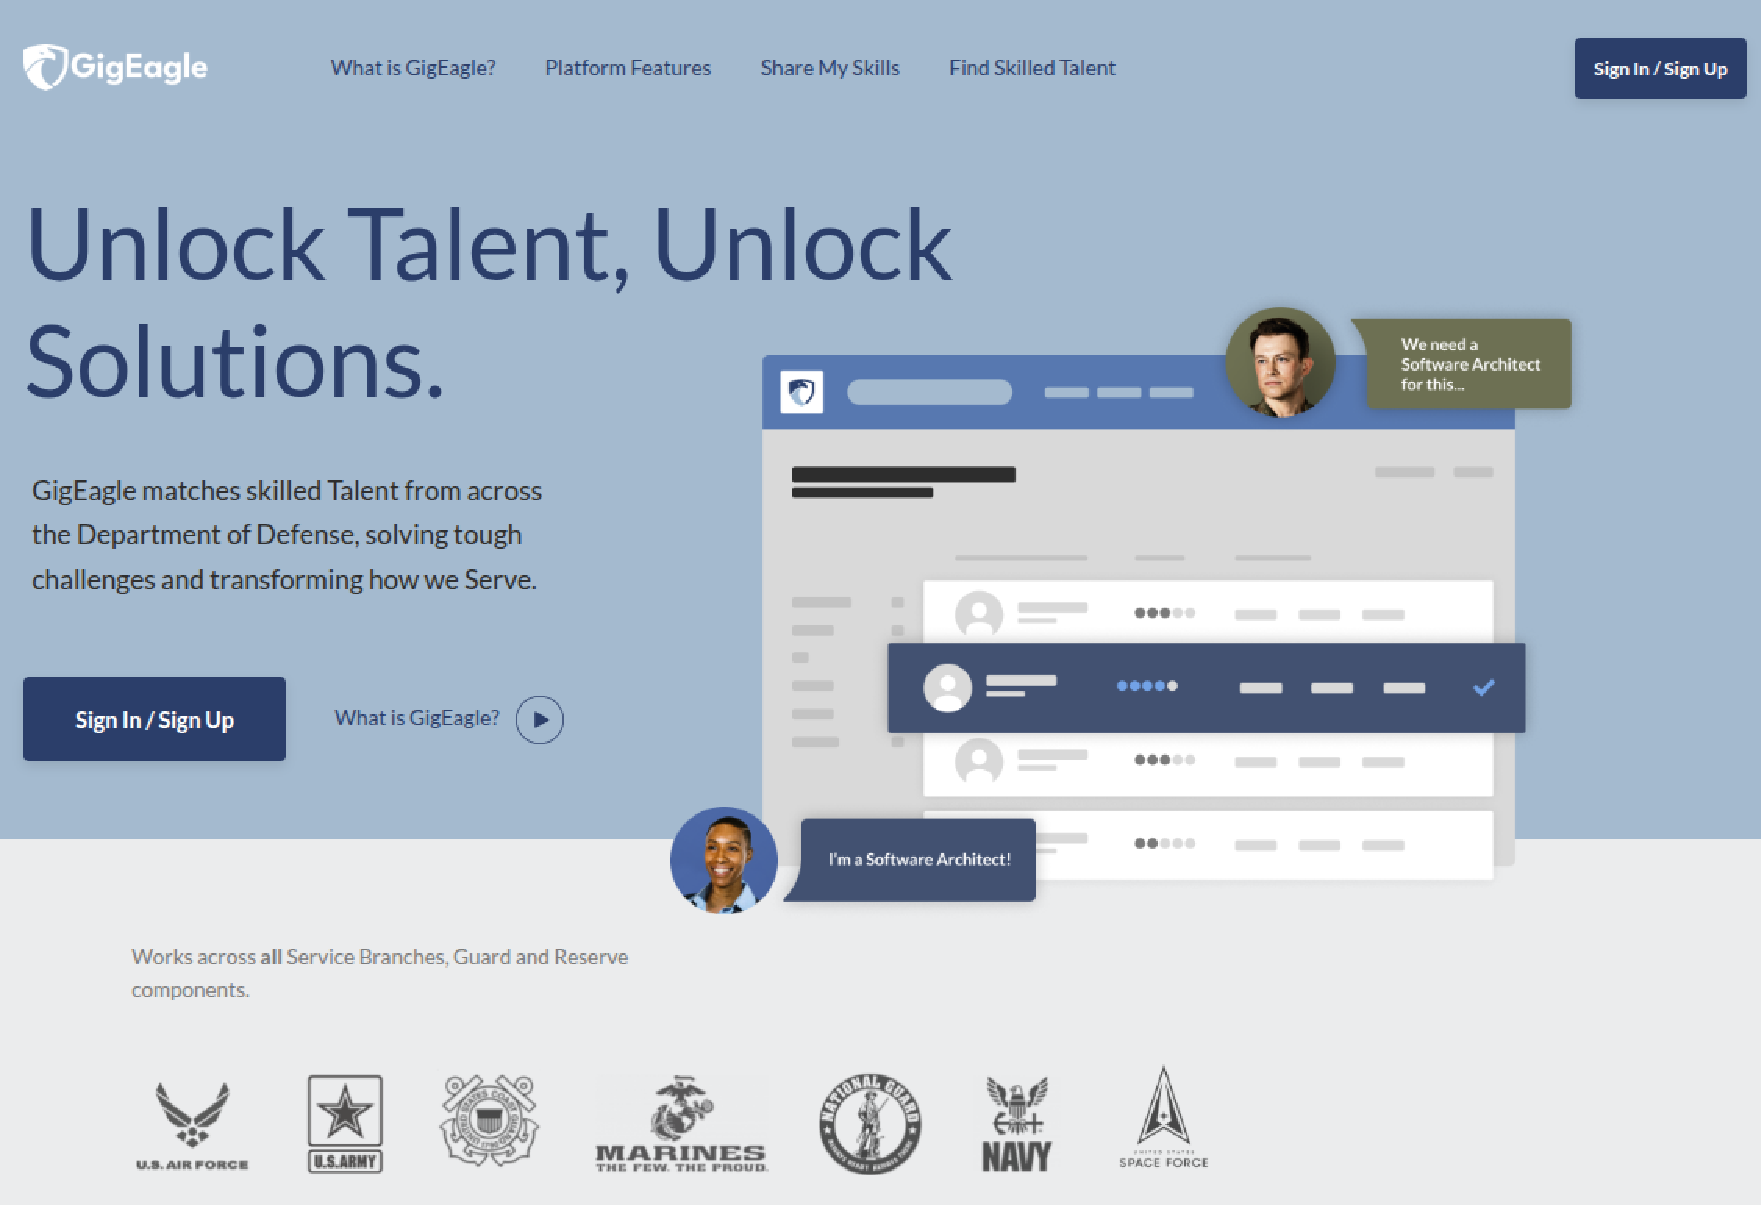
\includegraphics[width=\linewidth]{figures/gigeagle.pdf}
                \end{figure}
          \end{column}
        \end{columns}
      \end{frame}


      \begin{frame}{Conclusion}
        \begin{itemize}
          \item Lean/Six Sigma has gained traction in DoD and has been proves to be useful across DoD organization
          \item Lean implementation achieved through management practices, process improvements, continuous learning through data management
          \item Publication decline since is interesting 2017 suggests maturation in research, changing terminology, or maybe less adoption
        \end{itemize}
      \end{frame}

      \begin{frame}[allowframebreaks]{References}
        \footnotesize % Makes the text smaller
        \bibliographystyle{IEEEtran}
        \bibliography{/project/src/ref}
      \end{frame}
      
      \lastslide
\end{document}